
\documentclass[10pt]{article} % For LaTeX2e
\usepackage[preprint]{tmlr}
% If accepted, instead use the following line for the camera-ready submission:
%\usepackage[accepted]{tmlr}
% To de-anonymize and remove mentions to TMLR (for example for posting to preprint servers), instead use the following:
%\usepackage[preprint]{tmlr}

% Optional math commands from https://github.com/goodfeli/dlbook_notation.

\usepackage{hyperref}
\usepackage{url}
\usepackage{graphicx}
\usepackage{caption}
\usepackage{subcaption}


\title{Can Feature-Attainment Options Help for Multi-Task,\\Transfer, and Continual Reinforcement Learning?}

% Authors must not appear in the submitted version. They should be hidden
% as long as the tmlr package is used without the [accepted] or [preprint] options.
% Non-anonymous submissions will be rejected without review.

\author{\name Oliver Diamond  \\
      \addr Department of Computer Science\\
      University of Alberta, RLAI
      \AND
      \name Hector Kohler  \\
      \addr Universit\'e de Lille \\
      Inria
      \AND
      \name Adam White \\
      \addr Department of Computer Science \\
      University of Alberta, RLAI\\
      Amii Fellow \\
      CIFAR Fellow}

% The \author macro works with any number of authors. Use \AND 
% to separate the names and addresses of multiple authors.

\newcommand{\fix}{\marginpar{FIX}}
\newcommand{\new}{\marginpar{NEW}}



\begin{document}


\maketitle

\section{Background}
The bare minimimun for an artifical intelligence (AI) should be to accomplish one specific task in a specific environment.
For example, we hope that our cleaning robots can at least remove dust (one task) in a house (one environment).
For a single AI to be truely useful, it ought to do more than one single cleaning task and/or in more than one environment.
For example we would like our cleaninig robots to remove dust, but also stains and hair (multiple tasks), potentially in schools or hospitals (multiple environments).
We can even expect a cleaning robot to be easily re-purposed to do factory mapping, package carrying, robot racing, etc.
However we should not expect our cleaning robot to work underwater as it is a complete different world.
Most importantly, because the environments are uncertain, e.g., maybe the tenants moved the sofa yesterday, we want robots to adapt to their environment.

\textbf{Reinforcement learning} agents are algorithms that can train an AI to act and adapt to accomplish such task(s) through interaction with the environment(s).
\textbf{Multi-task reinforcement learning} agents train an AI that can accomplish a set of similar tasks in a given environment.
\textbf{Transfer reinforcement learning} agents re-purpose an AI to accomplish completely new tasks and/or to work in different environments.
\textbf{Continual reinforcement learning} agents continuously train an AI to accomplish new tasks while making sure previous tasks are not forgotten.
\textbf{Deep reinforcement learning} agents train an AI that rely implicitely on intermediate representations of the environments to take actions rather direcly relying on sensors or observations.
It is fair to compare those intermediate representations as an AI's ``understanding'' of the world.

In this document, we ask if multi-task, transfer and continual deep reinforcement learning agents are more efficient if the trained AI can explicitely interact with its intermediate representations.

\section{Worlds, Environments, and Tasks}
Before providing mathematical formalism; we illustrate with toy examples the notions of world, environment, and tasks.
All the figures presented in this sections are taken from the article \textit{Minigrid \& Miniworld: Modular \& Customizable Reinforcement Learning Environments for Goal-Oriented Tasks}, 2023, by Chevalier et. al. .
\begin{figure}
\centering
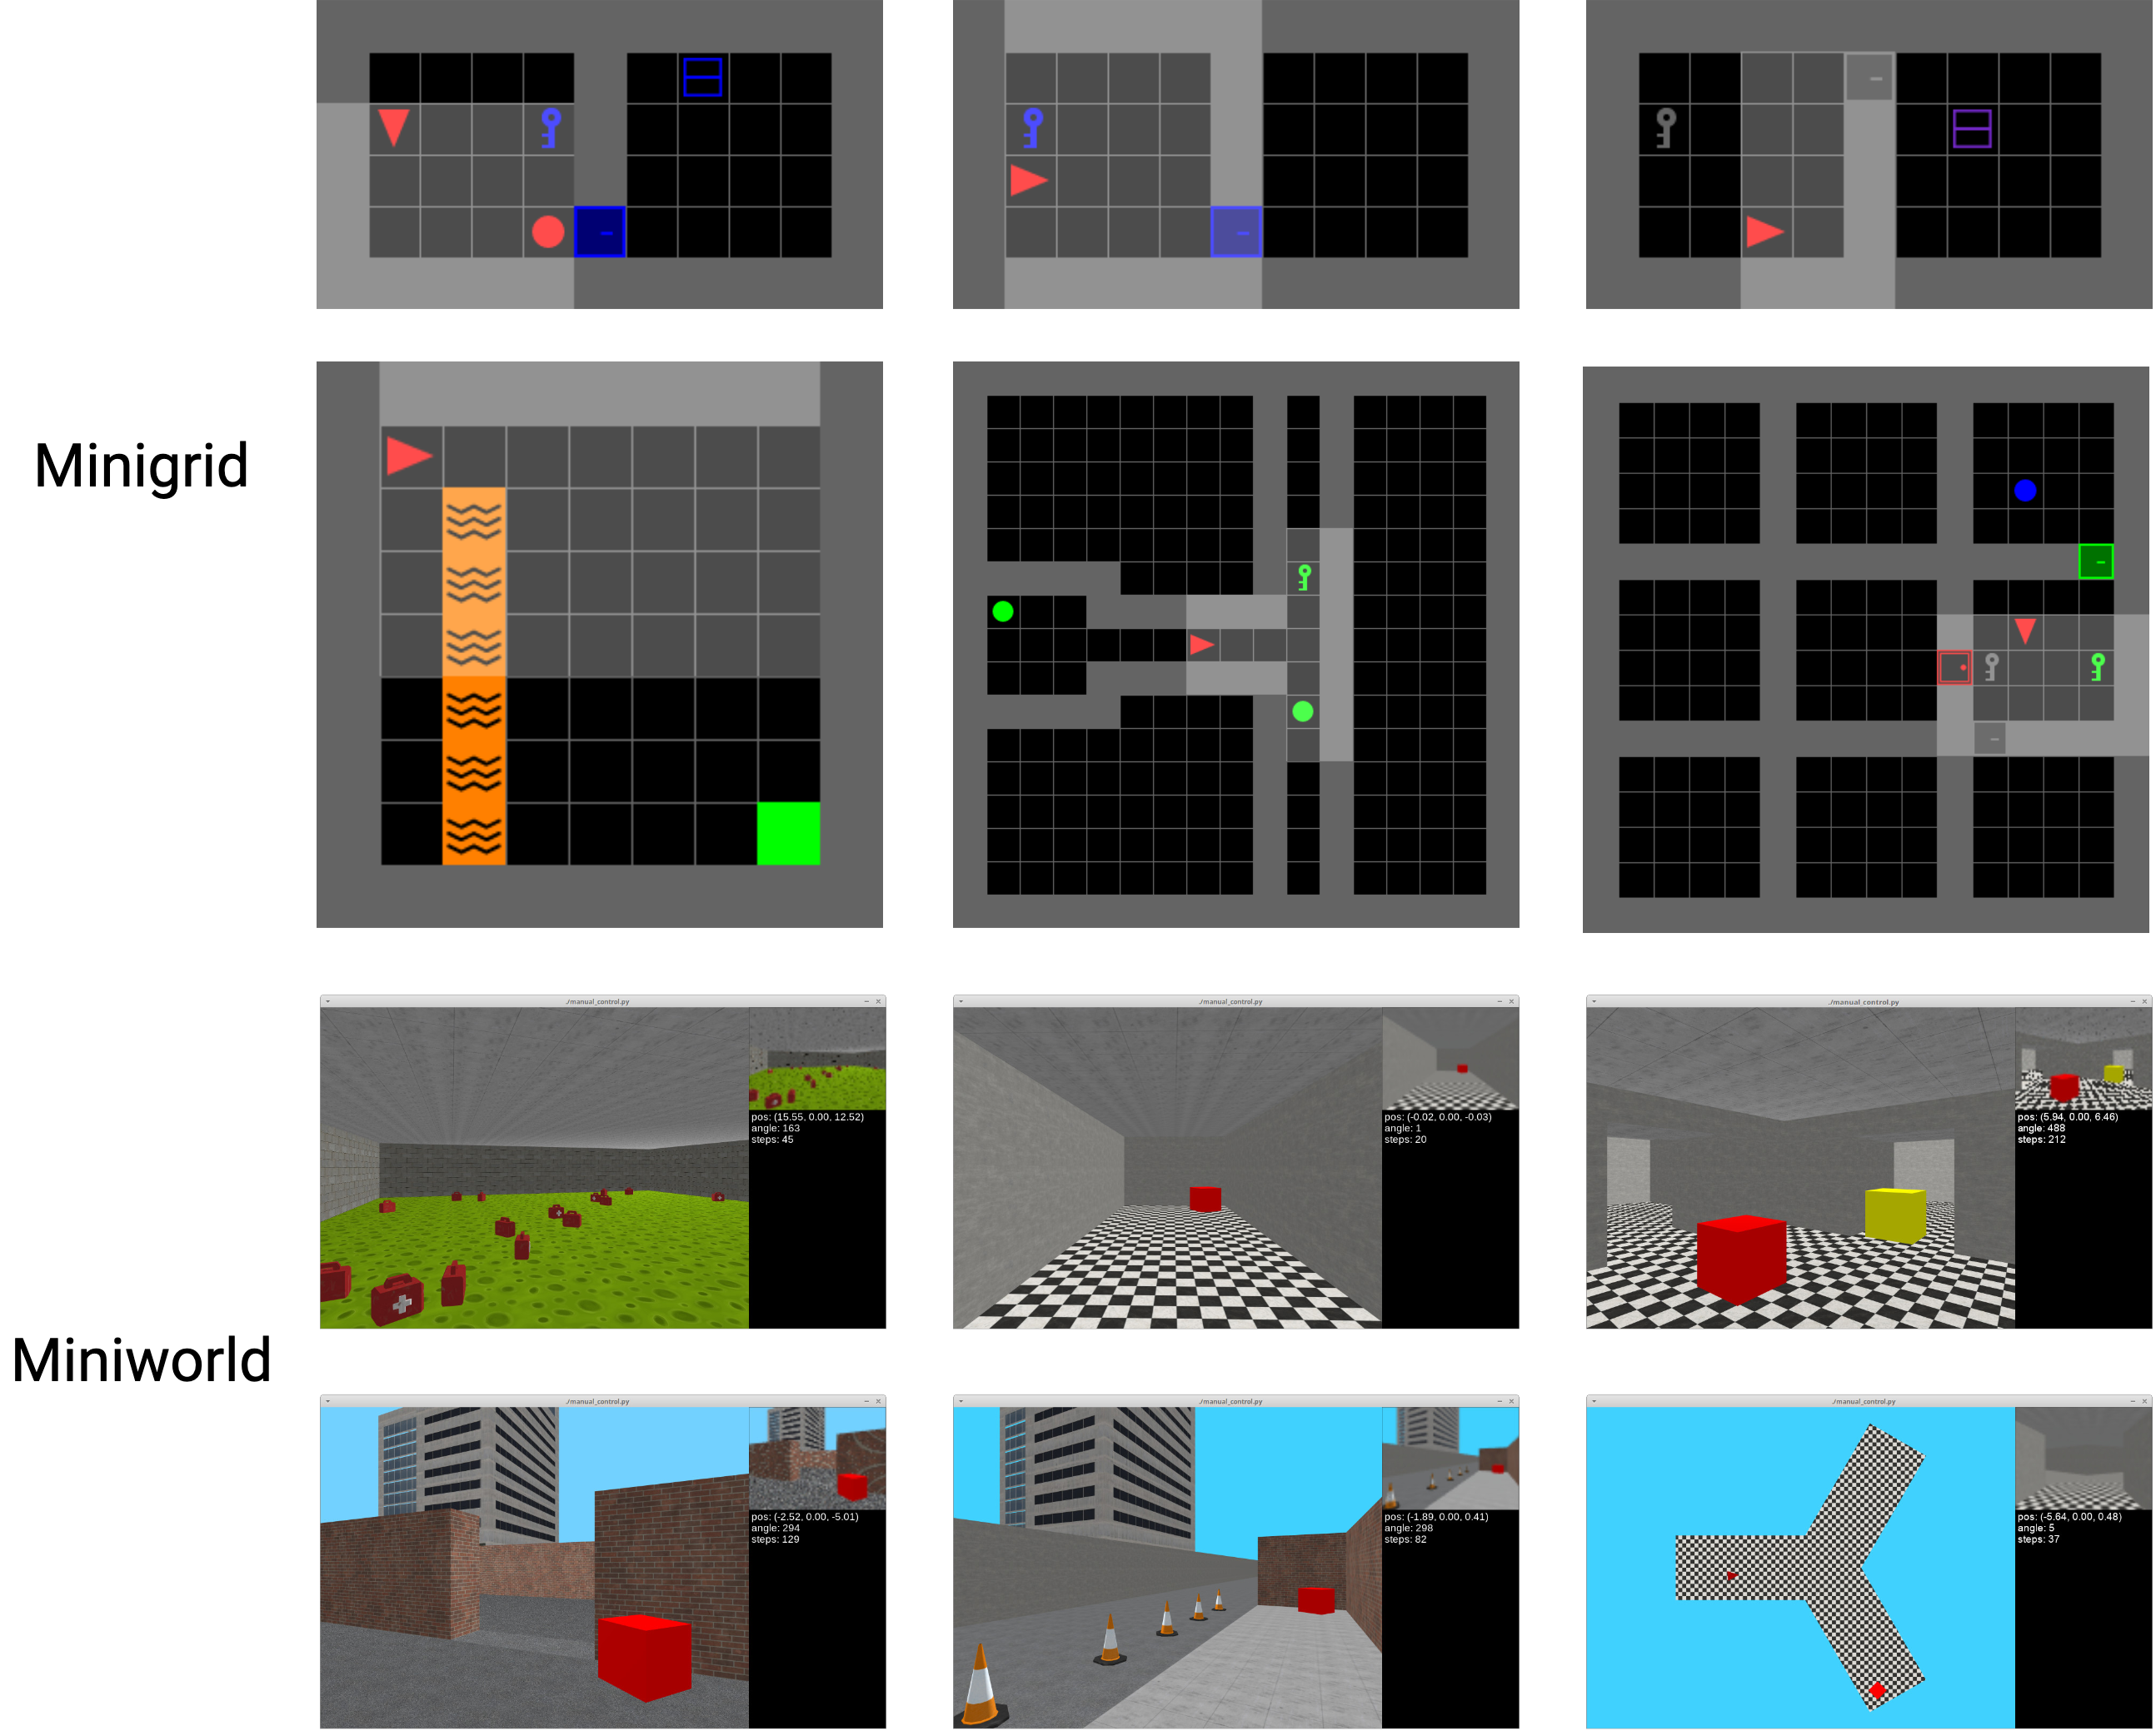
\includegraphics[width=0.7\textwidth]{figures/minigrid_miniworld_alt.png}
\caption{\textbf{Different worlds, different environments and different tasks}. (Top six rows) a 2D world with different environments and different tasks.
(Bottom rows) a 3D world with different environments and tasks.}
\end{figure}

\begin{figure}
  \centering
  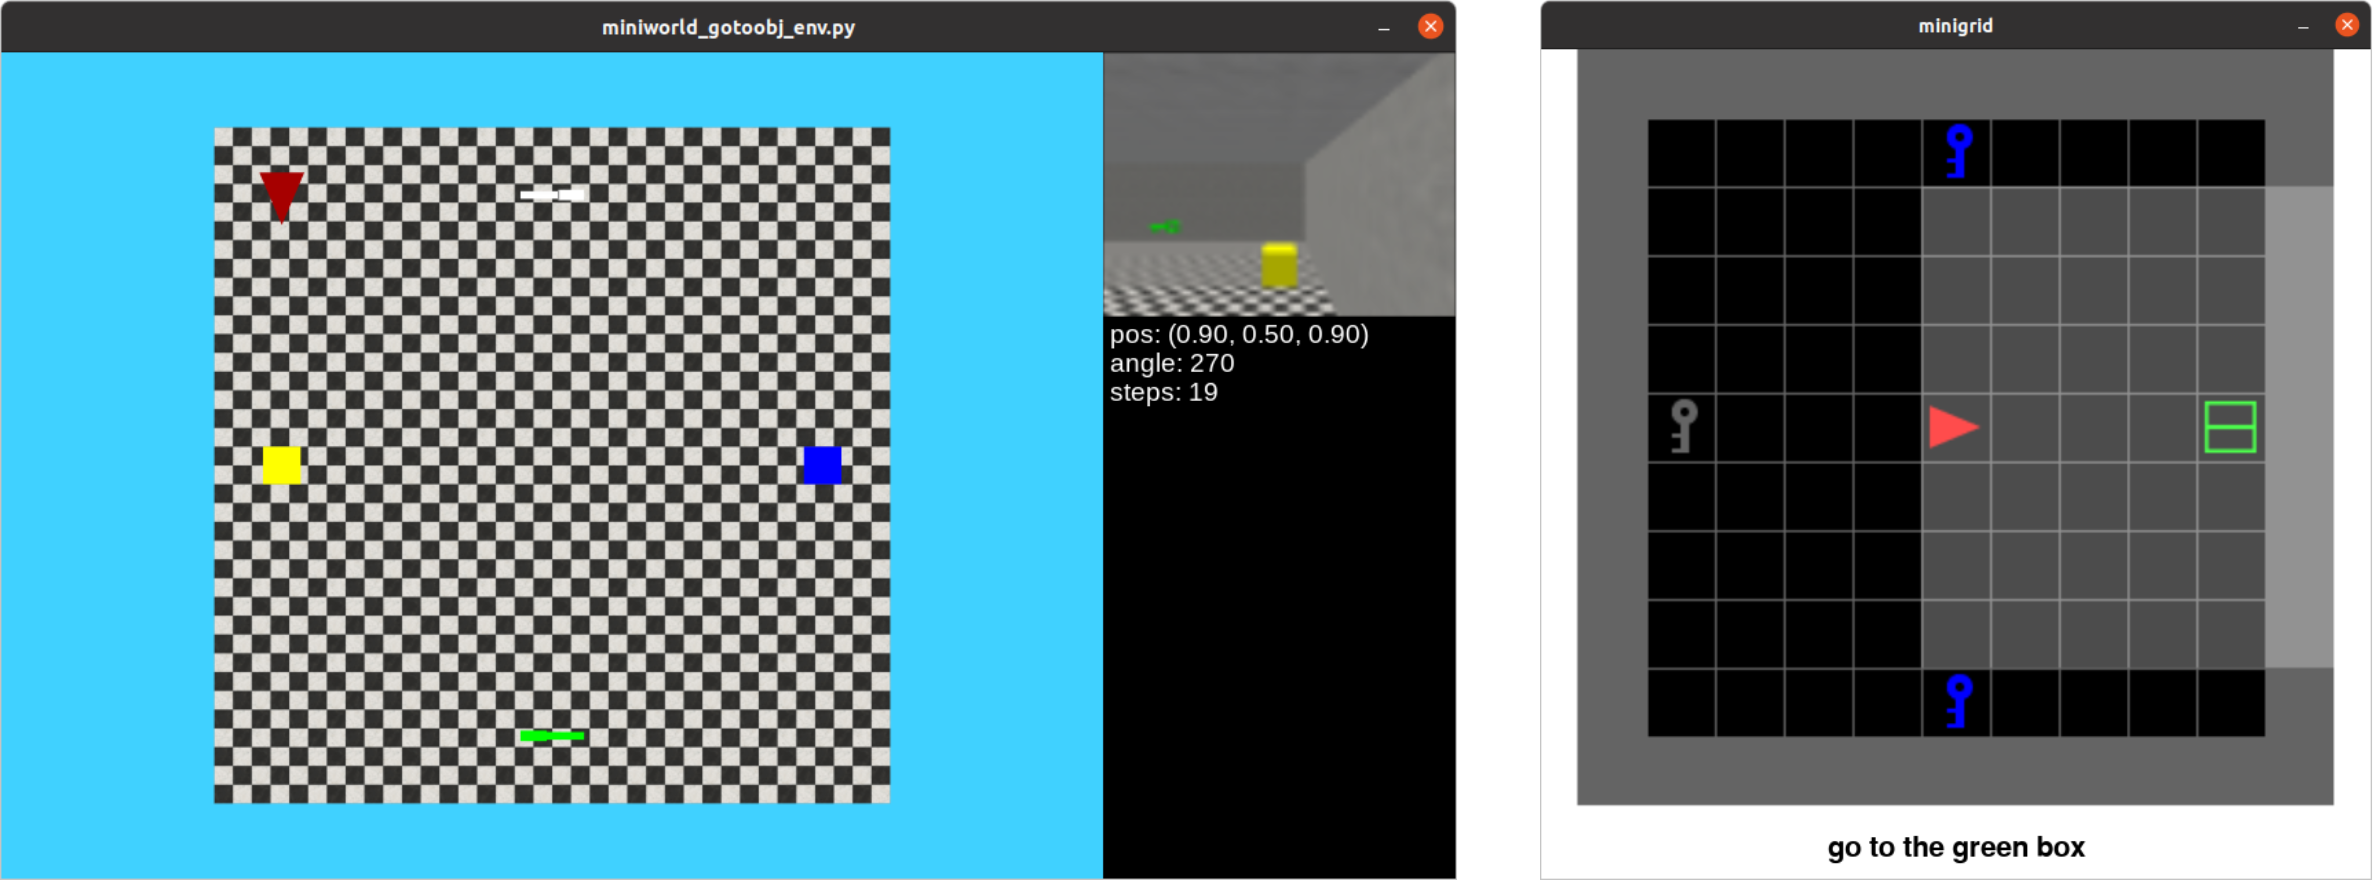
\includegraphics[width=0.7\textwidth]{figures/transfer_envs.png}
  \caption{\textbf{Different worlds and environments, same task}. (Left) an environment in a 3D world. (Right) an environment in a 2D world. 
  In both environments the AI needs to go to the green object.
  }
  \end{figure}


  \begin{figure}
    \centering
    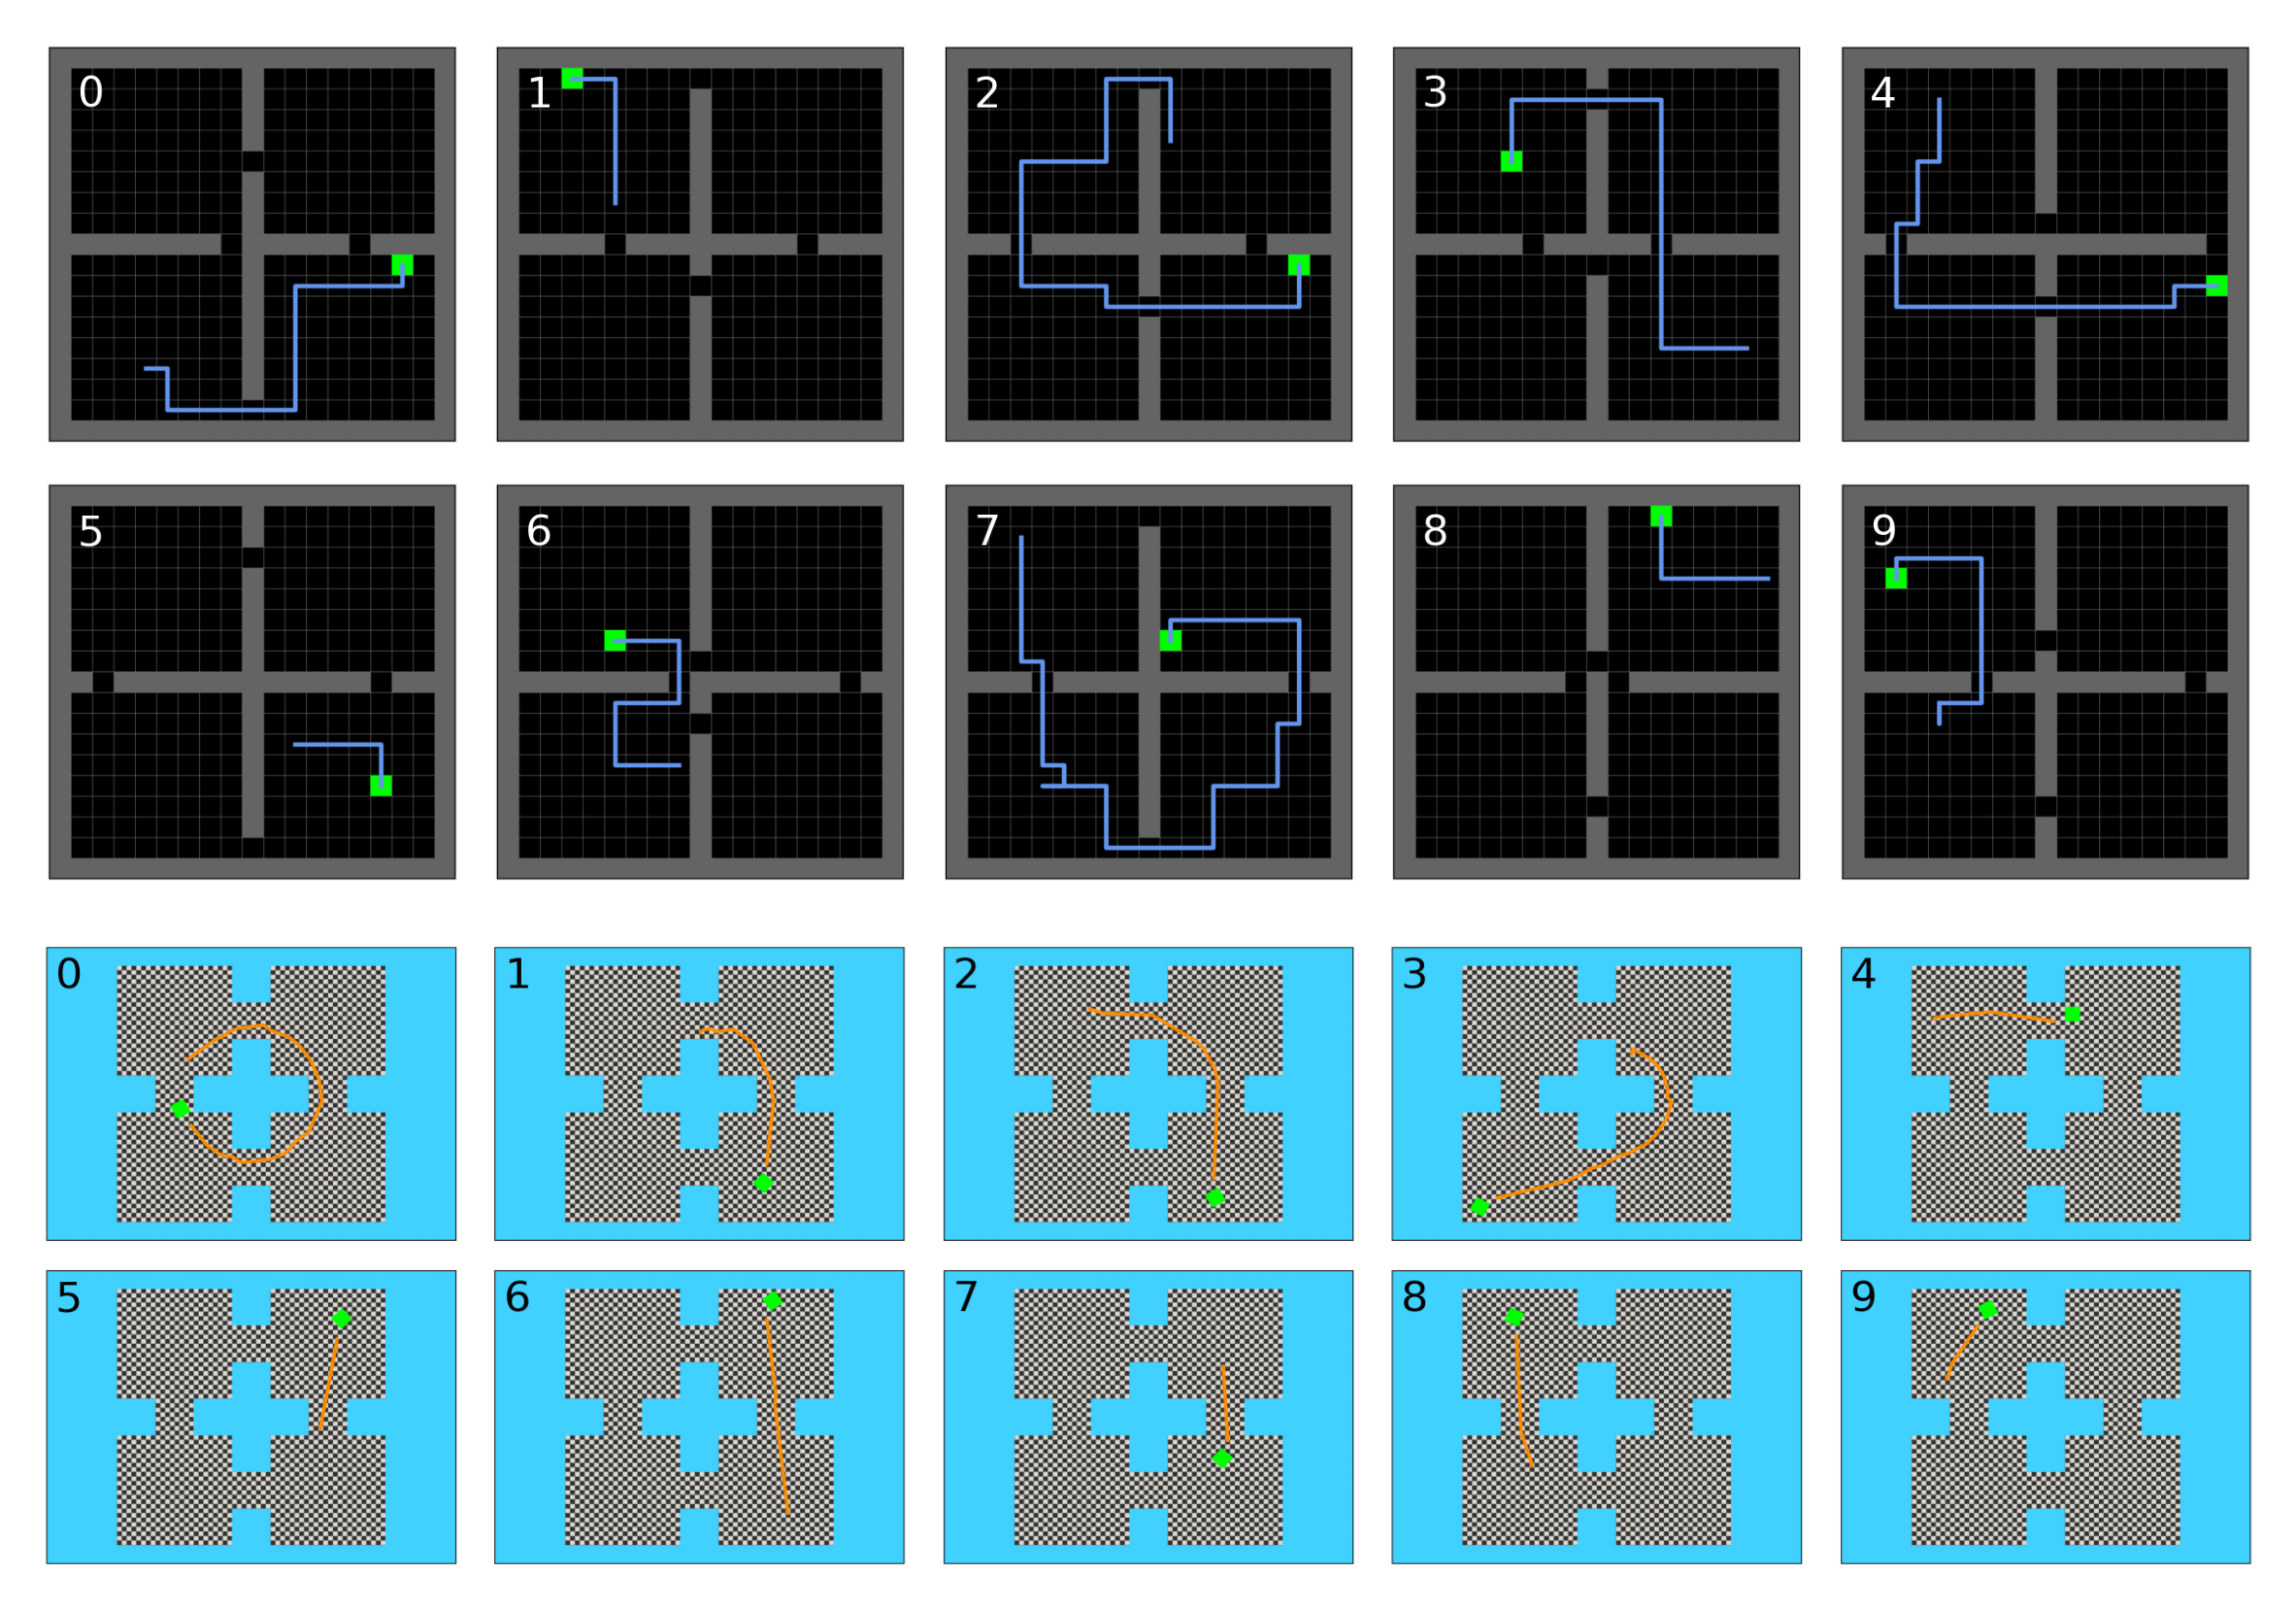
\includegraphics[width=0.7\textwidth]{figures/test_20230521-213858_20230521-214352.png}
    \caption{\textbf{Same world, different environments, same task}. (Top) a four-rooms house in a 2D world where the AI needs to reach the green square.
    (Bottom) an other house in the same 2D world where the AI also needs to reach the green square.} 
    \end{figure}


    \begin{figure}
      \centering
      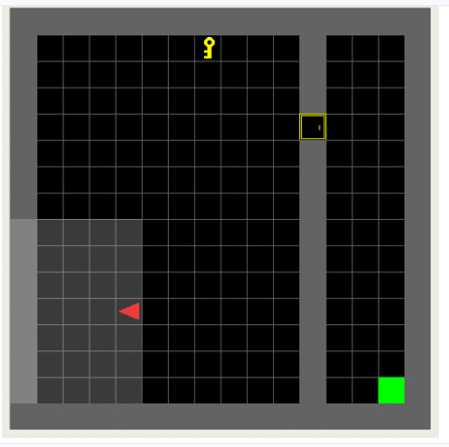
\includegraphics[width=0.5\textwidth]{figures/same_1.png}
      \caption{\textbf{Single environment, single task}. A two-rooms house where the AI needs to open the door and go to the green square.} 
      \end{figure}
  \begin{figure}
    \centering
    \begin{subfigure}[b]{0.45\textwidth}
    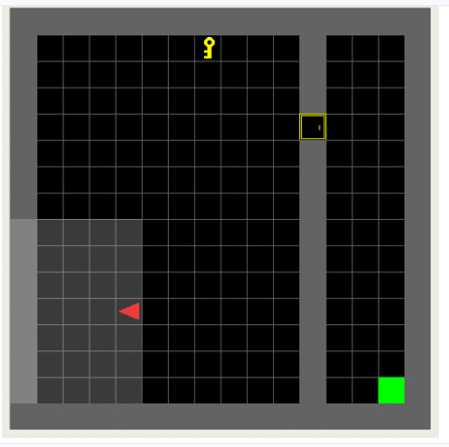
\includegraphics[width=1\textwidth]{figures/same_1.png}
    \end{subfigure}
    \begin{subfigure}[b]{0.45\textwidth}
      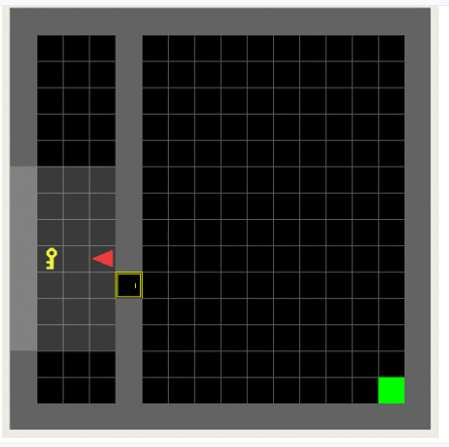
\includegraphics[width=1\textwidth]{figures/same_2.png}
      \end{subfigure}
    \caption{\textbf{Same (uncertain) environment, same task}. A two-rooms house, where the wall position changes randomly between each day, where the AI needs to open the door and go to the green square.} 
    \end{figure}

  \begin{figure}
    \centering
    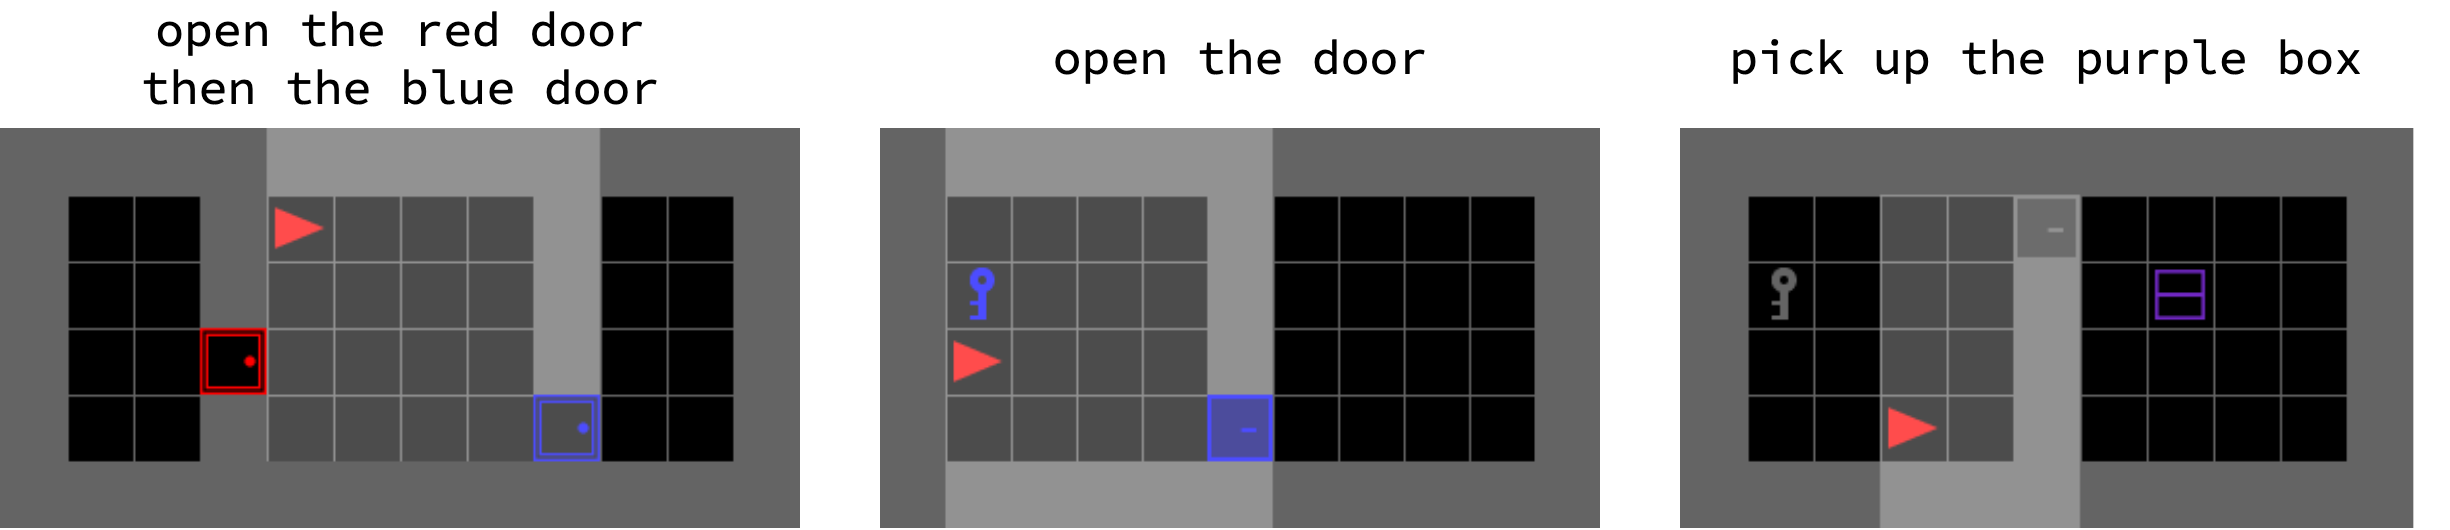
\includegraphics[width=0.9\textwidth]{figures/Minigrid_mission.png}
    \caption{\textbf{Same (uncertain) environment, different tasks}. (Left and centre) a two-rooms, house where walls can appear and disappear, the AI needs to open doors of different colors or to open locked doors. 
    This is a typical multi-task AI that can accomplish similar but different tasks. 
    (Right) the same two-rooms uncertain house where an AI has to pick up the purple box.
    A transfer learning agent could typically re-purpose the door-opening AI to pick up the box, while a continual learning agent could train the AI to pick up the box while making sure it can still open doors.}
    \end{figure}
\end{document}
